\section{Frequency mode 02}
\label{sec:fm02}

\subsection{Overview}
\label{sec:fm02:overview}
Frequency mode~02 monitors the band $544.102$--$544.902\,\mathrm{GHz}$. Its
main use is retrievals of \chem{O_3} and \chem{HNO_3}.

\TODO{General text about FM02}
\TODO{Show spectra?}

\subsection{Comparison of retrieved profiles}
\label{sec:fm02:comparison}
\TODO{Averaging kernels}


%%%%%%
% O3 %
%%%%%%

\begin{figure}[htpb]
    \centering
    \begin{subfigure}[b]{0.49\textwidth}
        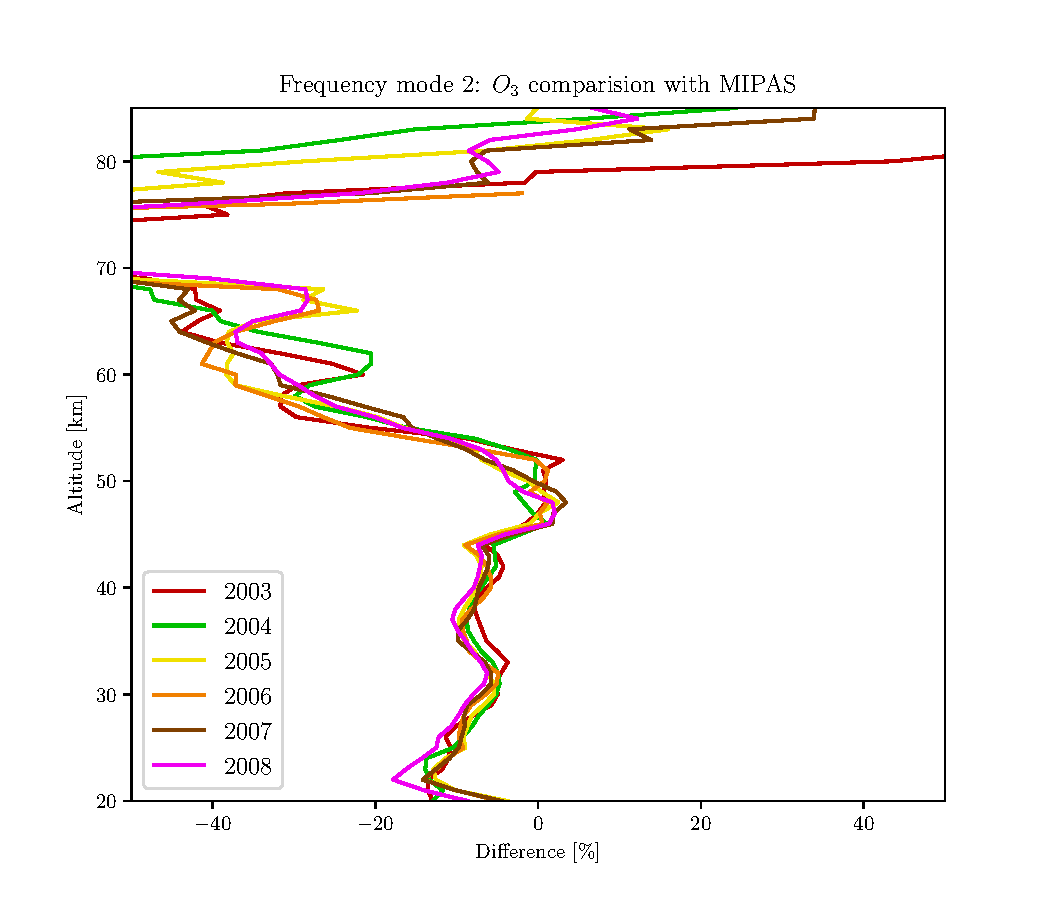
\includegraphics[width=\textwidth]{DDS_fm2_O3_perdiff_mipas}
        \caption{average difference to MIPAS}
        \label{fig:fm02:O3:profiles:MIPAS}
    \end{subfigure}
    \,
    \begin{subfigure}[b]{0.49\textwidth}
        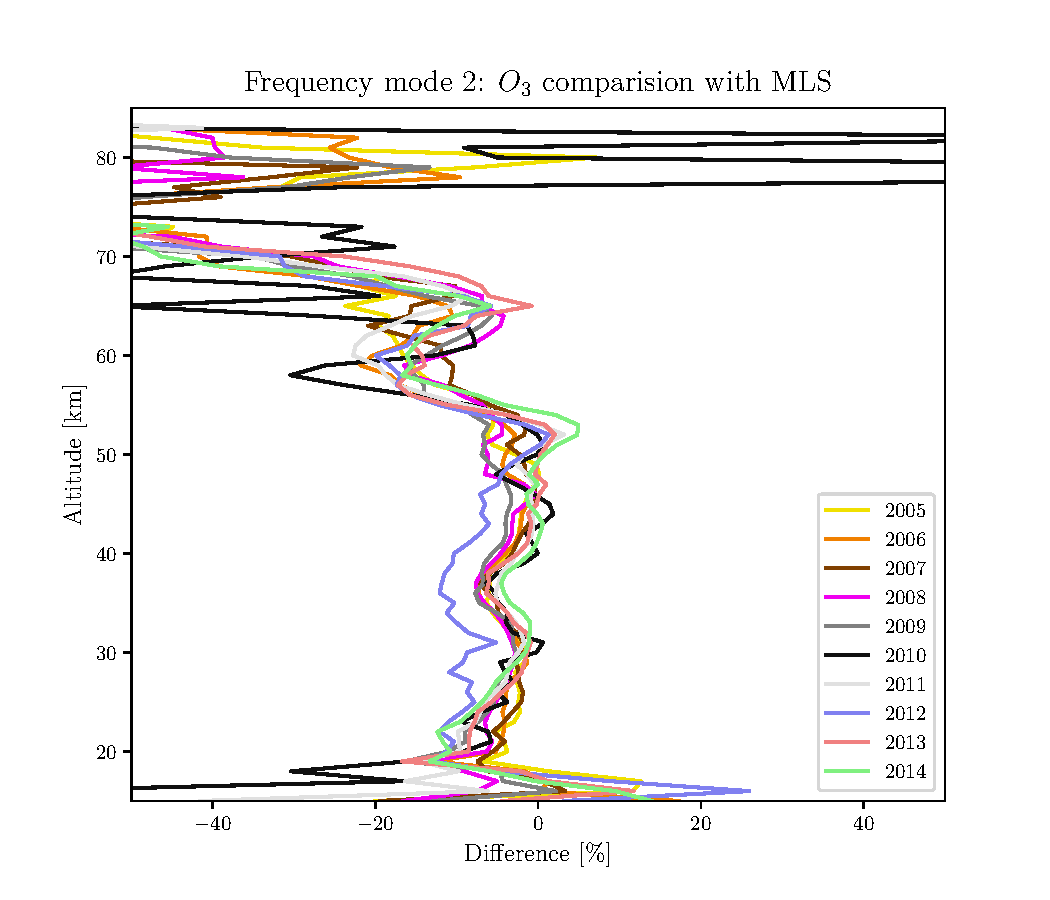
\includegraphics[width=\textwidth]{DDS_fm2_O3_perdiff_mls}
        \caption{average difference to MLS}
        \label{fig:fm02:O3:profiles:MLS}
    \end{subfigure}

    \begin{subfigure}[b]{0.49\textwidth}
        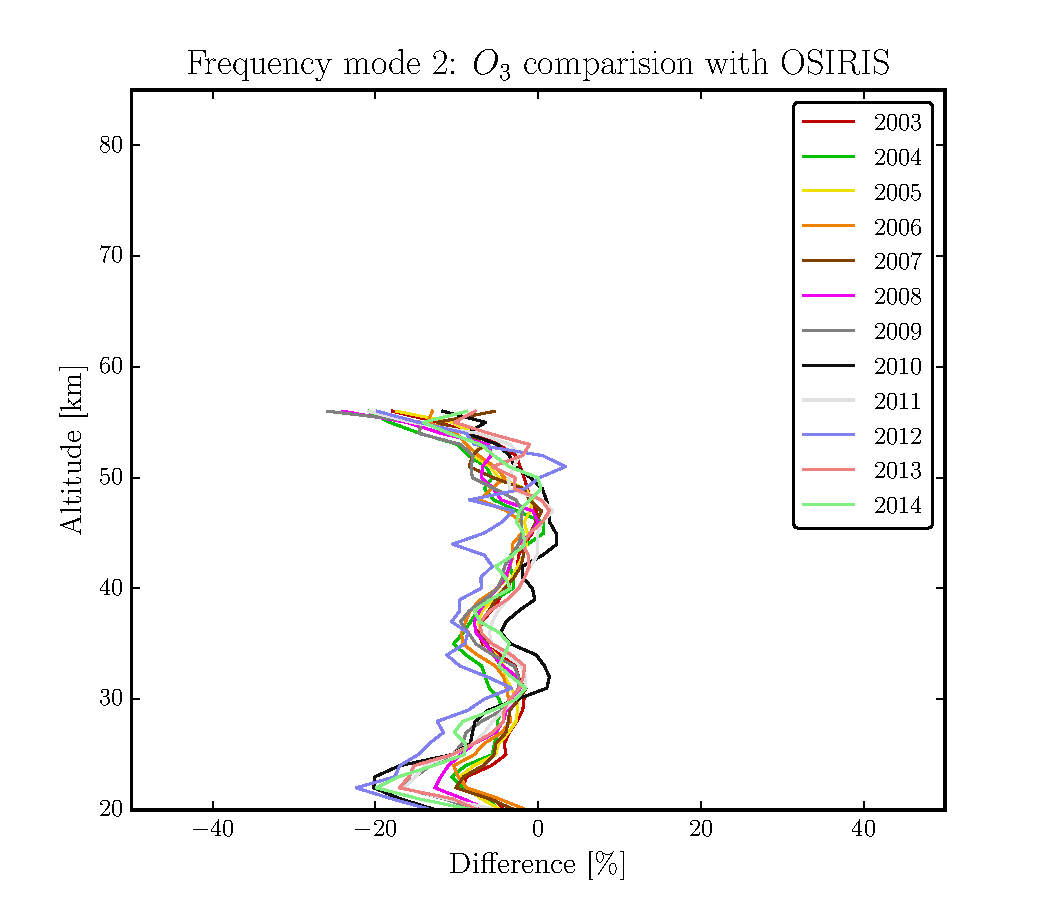
\includegraphics[width=\textwidth]{DDS_fm2_O3_perdiff_osiris}
        \caption{average difference to OSIRIS}
        \label{fig:fm02:O3:profiles:OSIRIS}
    \end{subfigure}
    \,
    \begin{subfigure}[b]{0.49\textwidth}
        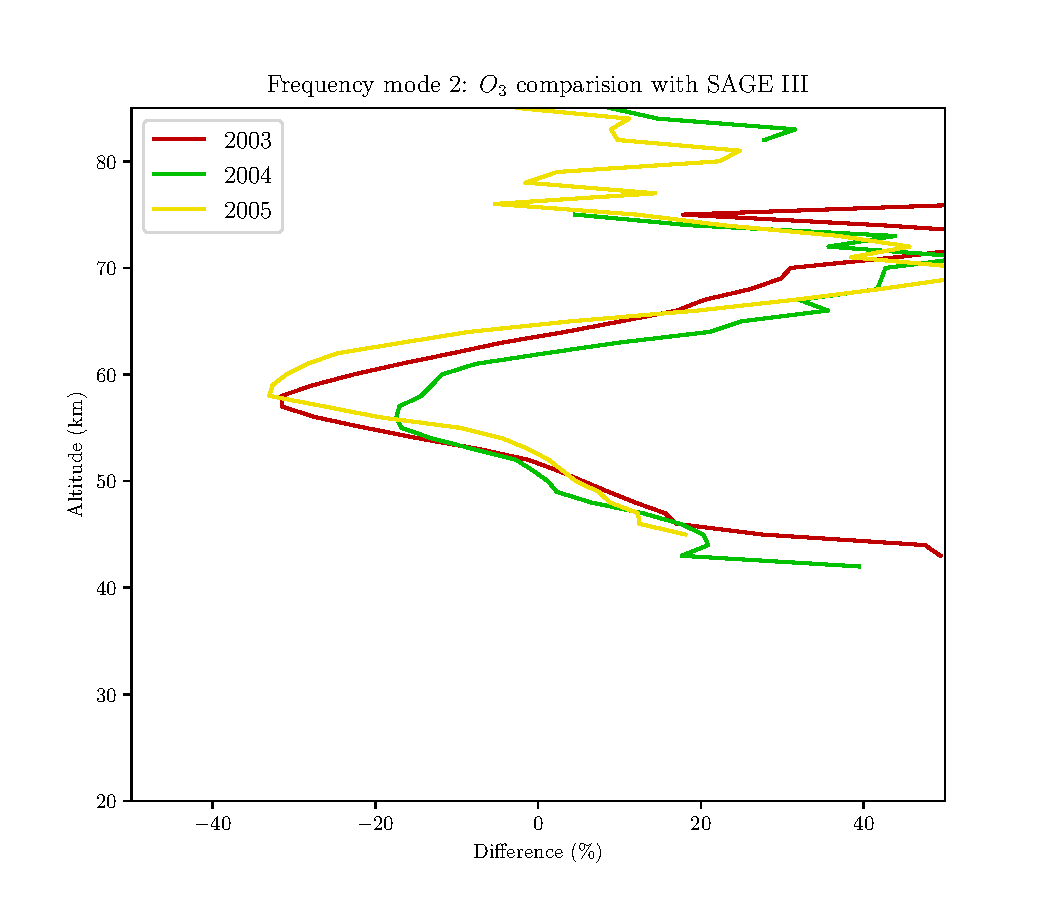
\includegraphics[width=\textwidth]{DDS_fm2_O3_perdiff_sage}
        \caption{average difference to SAGE~III}
        \label{fig:fm02:O3:profiles:SAGEIII}
    \end{subfigure}
    \caption{Average difference in percent between retrievals of \chem{O_3}
    from \smr~v3 and collocated measurements from various instruments at
    different altitudes for frequency mode~02. (Retrievals yielding
    concentrations $\leq 0.1\,\mathrm{ppm}$ have been filtered out.)}

    \label{fig:fm02:O3:profiles}
\end{figure}

\begin{figure}[htpb]
    \centering
    \begin{subfigure}[b]{0.49\textwidth}
        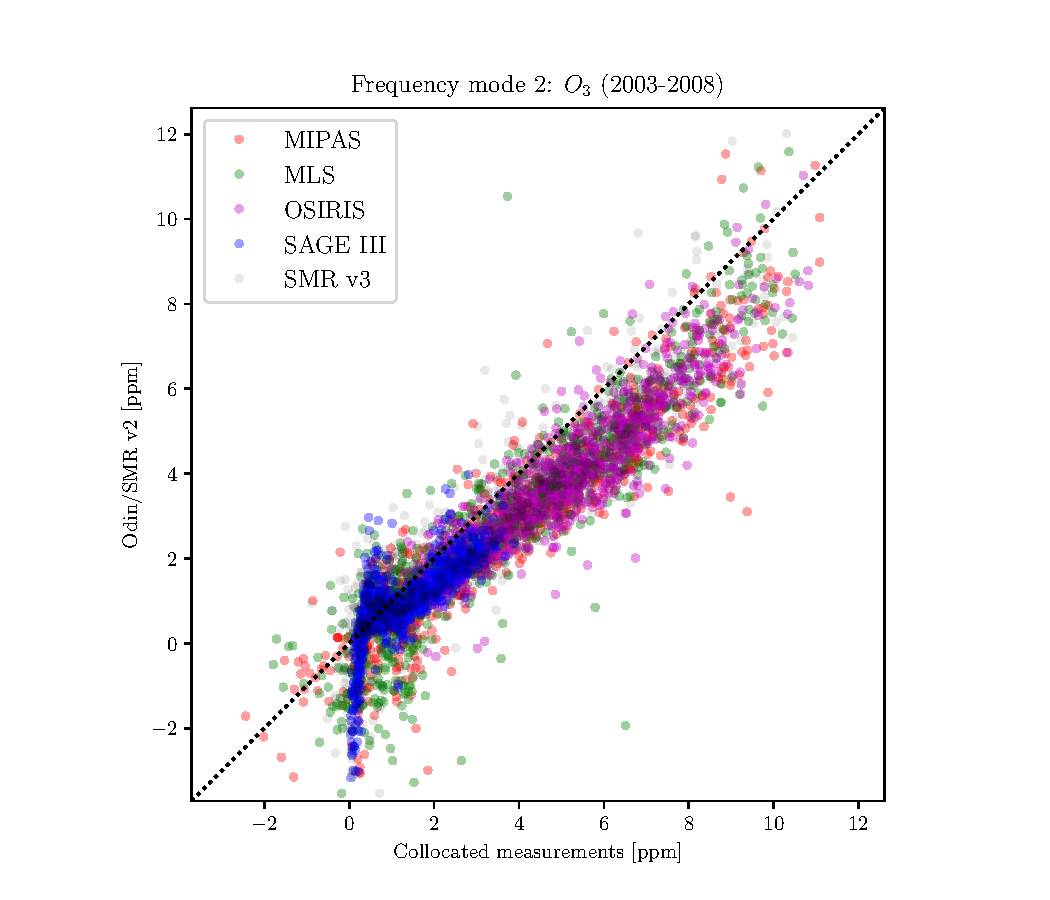
\includegraphics[width=\textwidth]{DDS_fm2_O3_scatter_v2}
        \caption{correlation of collcated instruments with \smr~v2.X}
        \label{fig:fm02:O3:scatter:v2}
    \end{subfigure}
    \,
    \begin{subfigure}[b]{0.49\textwidth}
        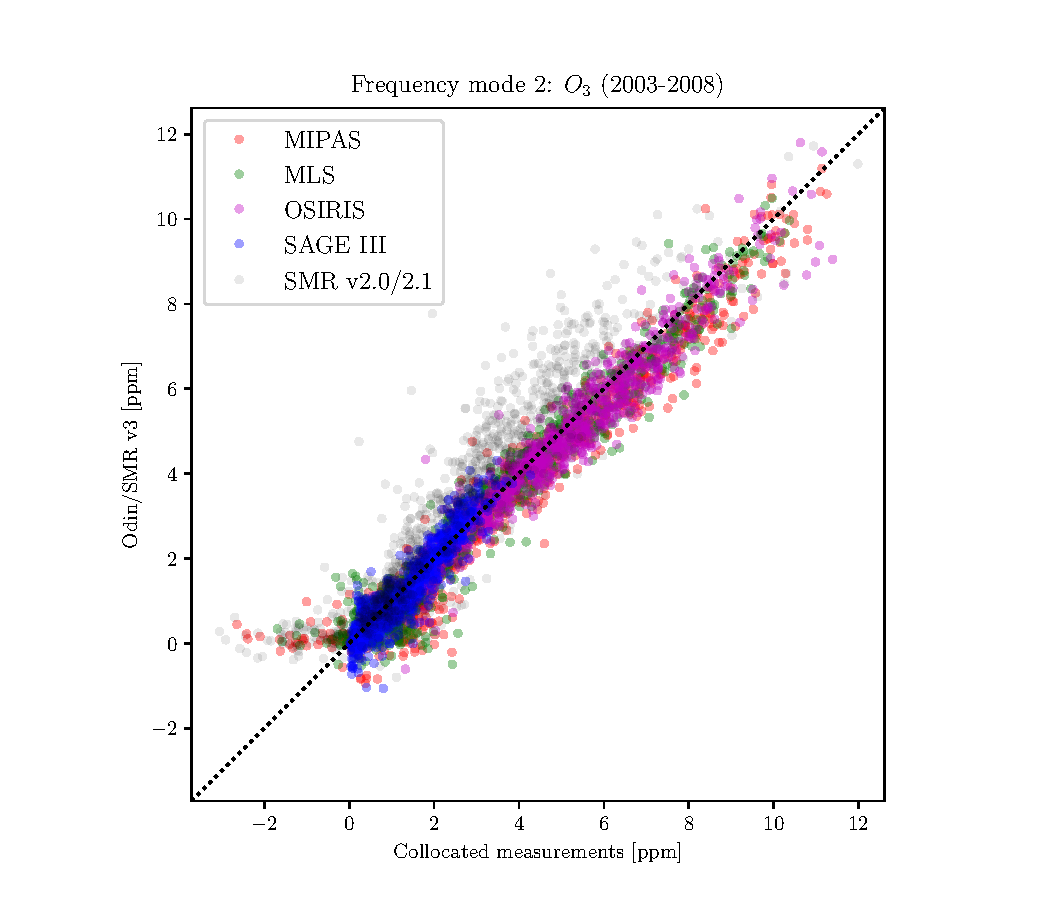
\includegraphics[width=\textwidth]{DDS_fm2_O3_scatter_v3}
        \caption{correlation of collcated instruments with \smr~v3}
        \label{fig:fm02:O3:scatter:v3}
    \end{subfigure}
    \caption{Correlation between retrievals of \chem{O_3} using \smr\
    versions~2.X and~3 and collocated measurements from various instruments
    for frequency mode~02.}
    \label{fig:fm02:O3:scatter}
\end{figure}

\subsubsection{\chem{O_3}}
\label{sec:fm02:comparison:O3}
The retrievals for \chem{O_3} have been compared with data from the MIPAS, MLS,
OSIRIS and SAGE~III instruments. Annual average differences to these
instruments are shown in Figure~\ref{fig:fm02:O3:profiles}. In
Figure~\ref{fig:fm02:O3:scatter} individual retrievals for the instruments for
the entire period are plotted agains the retrievals from the new and old
versions of the \smr\ processing chain. The results show a considerable
improvement with the updated version of the processing, with much better
over-all correlation and most of the systematic under estimation having been
removed compared to all the considered instruments. The largest improvement is
compared to SAGE~III, though, as seen in
Figure~\ref{fig:fm02:O3:profiles:SAGEIII}, there are still large systematic
differences depending on the altitude.


%%%%%%%%
% HNO3 %
%%%%%%%%

\begin{figure}[htpb]
    \centering
    \begin{subfigure}[b]{0.49\textwidth}
        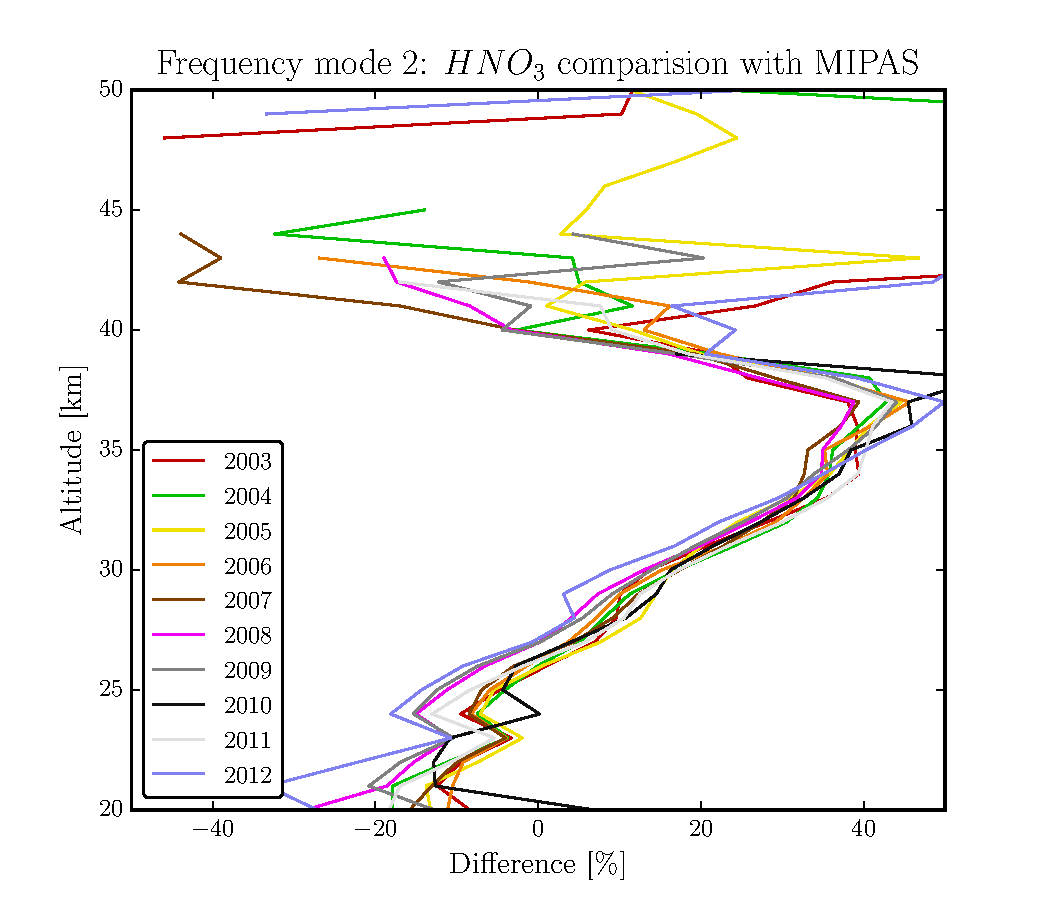
\includegraphics[width=\textwidth]{DDS_fm2_HNO3_perdiff_mipas}
        \caption{average difference to MIPAS}
        \label{fig:fm02:HNO3:profiles:MIPAS}
    \end{subfigure}
    \,
    \begin{subfigure}[b]{0.49\textwidth}
        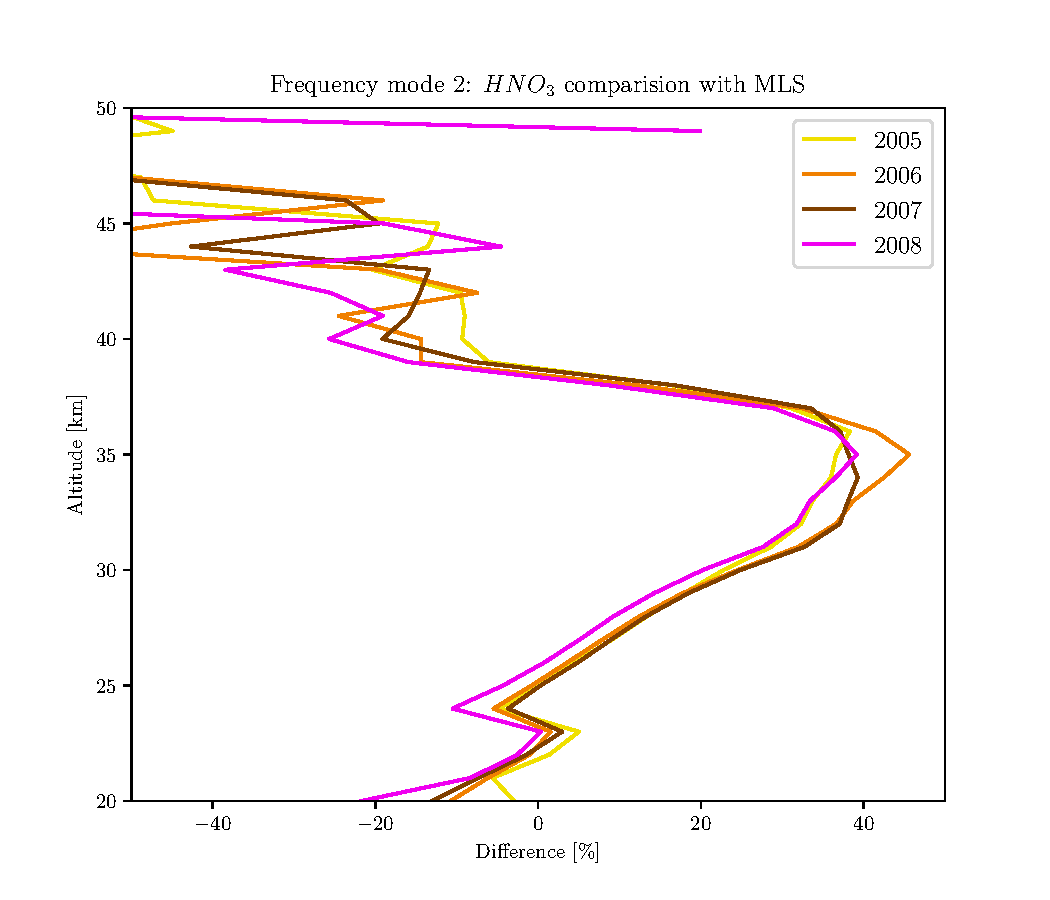
\includegraphics[width=\textwidth]{DDS_fm2_HNO3_perdiff_mls}
        \caption{average difference to MLS}
        \label{fig:fm02:HNO3:profiles:MLS}
    \end{subfigure}
    \caption{Average difference in percent between retrievals of \chem{HNO_3}
    from \smr~v3 and collocated measurements from various instruments at
    different altitudes. (Retrievals yielding concentrations
    $\leq 0.5\,\mathrm{ppb}$ have been filtered out.)}

    \label{fig:fm02:HNO3:profiles}
\end{figure}

\begin{figure}[htpb]
    \centering
    \begin{subfigure}[b]{0.49\textwidth}
        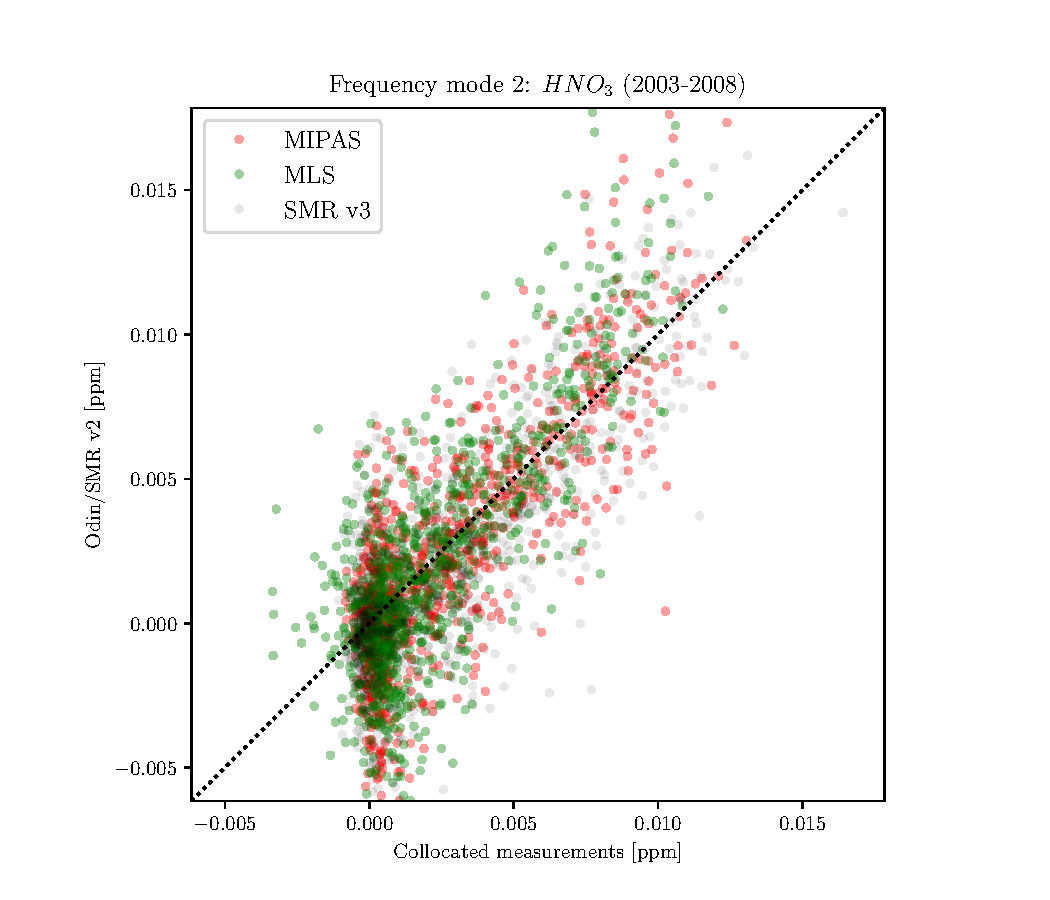
\includegraphics[width=\textwidth]{DDS_fm2_HNO3_scatter_v2}
        \caption{correlation of collcated instruments with \smr~v2.X}
        \label{fig:fm02:HNO3:scatter:v2}
    \end{subfigure}
    \,
    \begin{subfigure}[b]{0.49\textwidth}
        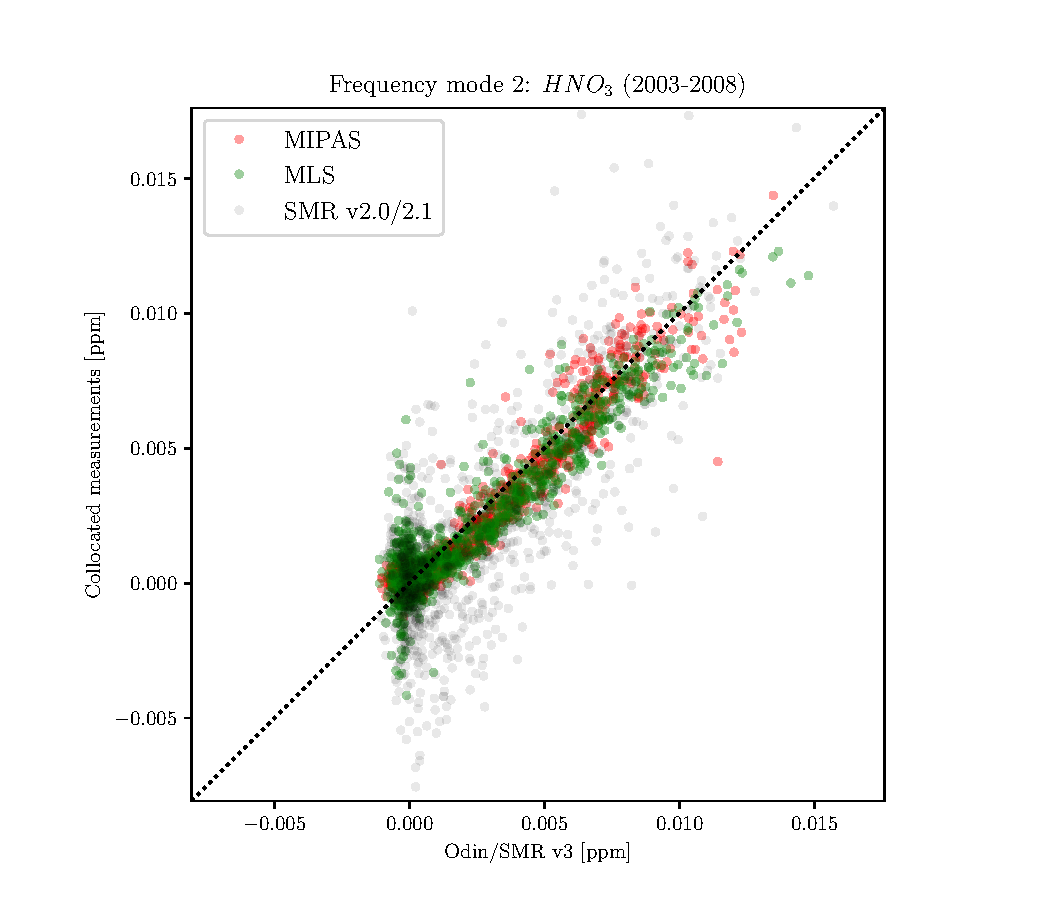
\includegraphics[width=\textwidth]{DDS_fm2_HNO3_scatter_v3}
        \caption{correlation of collcated instruments with \smr~v3}
        \label{fig:fm02:HNO3:scatter:v3}
    \end{subfigure}
    \caption{Correlation between retrievals of \chem{HNO_3} using \smr\
    versions~2.X and~3 and collocated measurements from various instruments.}
    \label{fig:fm02:HNO3:scatter}
\end{figure}

\subsubsection{\chem{HNO_3}}
\label{sec:fm02:comparison:HNO3} The retrievals for \chem{O_3} have been
compared with data from the MIPAS and MLS instruments. Annual average
differences to these instruments are shown in
Figure~\ref{fig:fm02:HNO3:profiles}. In Figure~\ref{fig:fm02:HNO3:scatter}
individual retrievals for the instruments for the entire period are plotted
agains the retrievals from the new and old versions of the \smr\ processing
chain. The results show a considerable improvement with the updated version of
the processing comapred to both considered instruments. The over-all
correlation is much better, though there are still large systematic differences
depending on the altitude, resulting in \smr\ over estimating the
concentrations.

\subsubsection{\chem{Temperature}}
\label{sec:fm02:comparison:temperature}
\TODO{Compare ??}


\subsection{Discussion}
\label{sec:fm02:discussion}
The Pearson correlation between the \smr\ retrievals and the other instruments
was calculated for the entire period for both versions of the processing chain.
The results are summarised in Table~\ref{tab:fm02:stats}, and show that the
new algorithm is a improvement compared to all the instruments for all species
used in this investigation. The improvement is considerable for both \chem{O_3}
and \chem{HNO_3}.


\begin{table}[hbt]
\centering
\caption{Pearson correlation and fit parameters of the old and new \smr\
retrievals for frequency mode~02, compared with collocated data from other
instruments for the period 2003--2008.
}
\label{tab:fm02:stats}
\begin{tabular}{lllrrrr}
    \toprule
    \textbf{Species} & \textbf{Instrument} & \textbf{SMR} & \textbf{corr.} & \textbf{slope} & \textbf{intercept} & \textbf{$\left|\left<\right.\right.$res.$\left.\left.\right>\right|$} \\
    \midrule
    \chem{O3}       & MIPAS     & v3    & 0.975 & 0.934 & -0.088\,ppm   & 0.692\,ppm \\
                    &           & v2.x  & 0.922 & 0.822 & -0.382\,ppm   & 1.458\,ppm \\
    \cline{2-7}
                    & MLS       & v3    & 0.973 & 0.946 & 0.028\,ppm    & 0.626\,ppm \\
                    &           & v2.x  & 0.903 & 0.846 & -0.347\,ppm   & 1.396\,ppm \\
    \cline{2-7}
                    & OSIRIS    & v3    & 0.973 & 0.947 & 0.047\,ppm    & 0.521\,ppm \\
                    &           & v2.x  & 0.900 & 0.810 & -0.171\,ppm   & 1.404\,ppm \\
    \cline{2-7}
                    & SAGE III  & v3    & 0.927 & 1.064 & -0.109\,ppm   & 0.393\,ppm \\
                    &           & v2.x  & 0.757 & 0.835 & -0.229\,ppm   & 0.790\,ppm \\
    \midrule
    \chem{HNO_3}    & MIPAS     & v3    & 0.967 & 0.989 & 0.184\,ppb    & 0.796\,ppb \\
                    &           & v2.x  & 0.810 & 1.051 & -0.411\,ppb    & 2.296\,ppb \\
    \cline{2-7}
                    & MLS       & v3    & 0.932 & 0.995 & 0.286\,ppb    & 1.148\,ppb \\
                    &           & v2.x  & 0.794 & 1.052 & 2.565\,ppb    & 2.565\,ppb \\
    \midrule
    Temp.           & MLS       & v3    & 0.952 & 0.937 & 13.343\,K     &  5.875\,K \\
                    &           & v2.x  & 0.794 & 0.700 & 66.058\,K     & 13.495\,K \\
    \bottomrule
\end{tabular}
\end{table}

\subsection{Conclusions}
\label{sec:fm02:conclusions}
\TODO{Recommended usage: which species, which periods}
Based on the discussion above, retrievals based on frequency mode~02 can be
used with confidence for the species \chem{O_3} and \chem{HNO_3} both.
